\section{Method}
%----------------------- Method ----------------------------
\label{sec:method}

In this section it will be described the steps and decisions taken towards the development of Sesnando. The concepts presented here are the result of the study of the state of the art and internal discussions with Project Advisors.


\subsection{Resource Analysis}
%----------------------- Resource Analysis ----------------------------
\label{subsec:resource_analysis}

This section presents the analysis procedures towards the available resources, namely, requirements sets. The Railway project used for this study stores its requirements on a Requirement Management Tool, it was needed to export such requirements and treat some data to extract relevant knowledge from them towards building a solid grammar that could satisfy these requirements logic.\\

It was not feasible to analyse such requirement one-by-one due to their ammount, so a tool has been developed to extract the needed data. First, the requirements have been exported in chunks of Excel files, but later, this same tool was able to directly access the requirement repository.

The requirement analysis tool has been developed using the following libraries.

\begin{itemize}
    \item pandas - For importing requirement files, data storage and data analysis.
    \item nltk - Natural Language Toolkit for data analysis.
    \item matplot - Data visualisation.
    \item xlswriter - To persist processed data.
\end{itemize}

The principal analysis taken was in the fields on the contiguous sequence and main requirement structures, for this, several models on N-Grams and Skip-grams have been generated.\\
N-gram model analysis are widely used in computational linguistics and communication theory such as Natural Language Processing (NLP) \cite{broder_syntactic_1997}.\\

The techniques to export the best N-gram models relied on arbitrary values and \textit{trial and error}. N-gram models above the value of 10 started to produce several repeating sequences, so the model analysis sat between the values of 2 and 10. Next is one of the N-gram Model where N = 10.

% width=\textwidth
\begin{figure}[H]
    \centering
    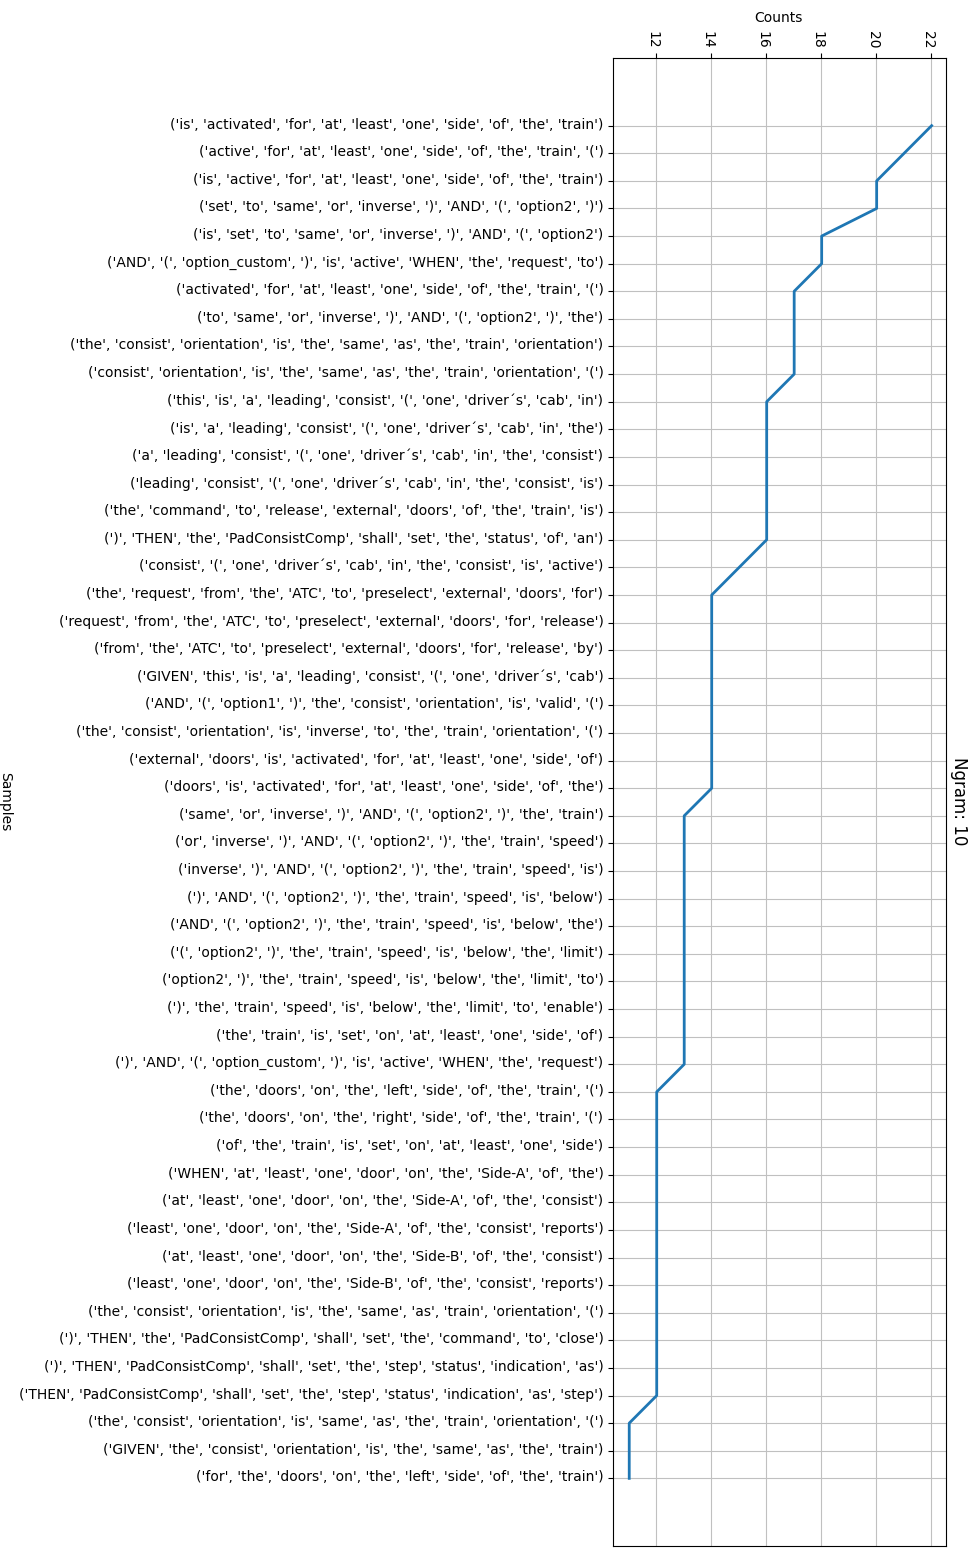
\includegraphics[scale=0.6]{images/n_gram10_cut.png}
    \caption{N-gram Model, N = 10}
    \label{fig:n_gram_model_10}
\end{figure}

The results of this analysis expressed the need of using boolean operators such as "AND" and "OR". Signal states such as "is active". Quantifiers containing their component/attribute and scope, as in "for at least one side of the train" and the \textit{THEN} condition in the form of "THEN the \textit{AUTOR} shall set the Requirement signal to \textit{VALUE}".
These have been used to define the requirements grammar, as it will be seen on next section (\ref{sec:def_req_grammar}).


\subsection{Defining the requirements grammar}
%----------------------- Defining the requirements grammar ----------------------------
\label{sec:def_req_grammar}

As the grammar lexer set has been identified it was then necessary to define an Abstract Syntax tree. It was known that the \textit{GIVEN}, \textit{WHEN} and \textit{THEN} where the main predicates that define the skeleton of a requirement, thus, each predicate should implement its own Condition tree.\\
There are widely known libraries to support the building of a grammar, such as Flex and Bison \cite{levine_flex_2009}, however, flex and bison only work with C++ programs and Antlr works with a number of different languages \cite{antlr_site}, hence, the choosing of Antlr library to support the development of this grammar. \textit{GIVEN}, \textit{WHEN} and \textit{THEN} are represented in the form of a Logical Expression that can be derived into child classes, given the lexer type. Next is the representation of the syntax tree (Fig. \ref{fig:ast_class_diagram}).

% 
\begin{figure}[H]
    \centering
    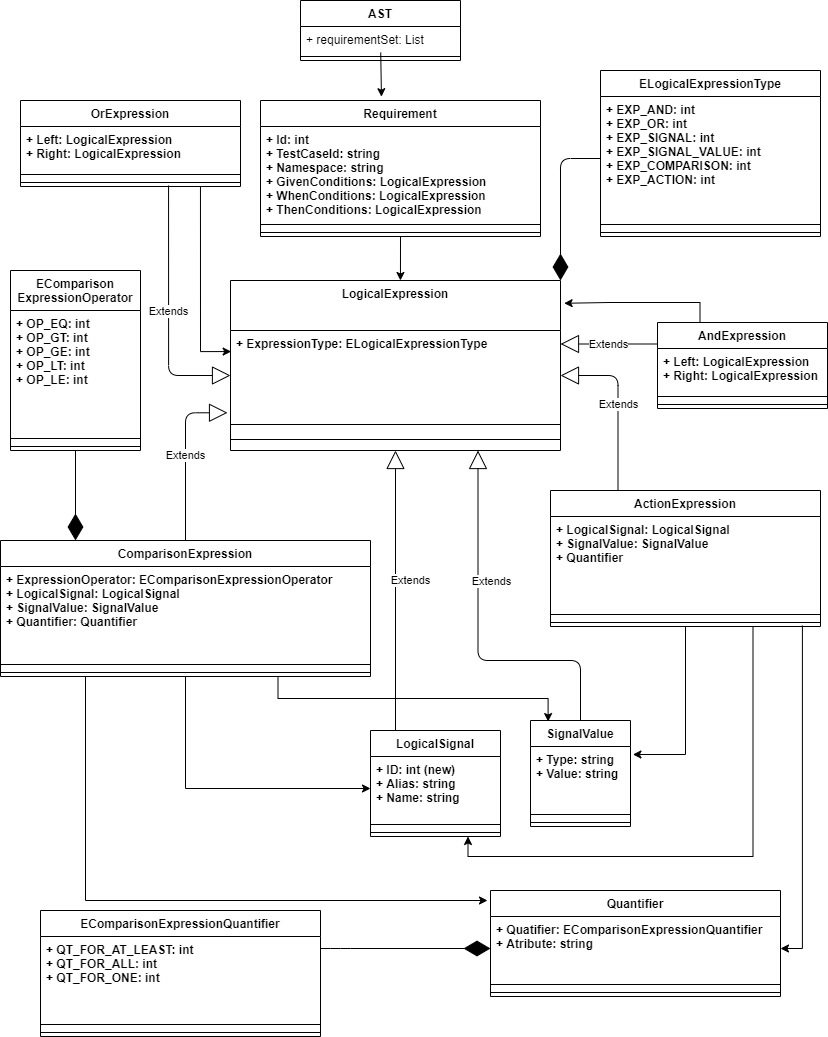
\includegraphics[width=\textwidth]{images/grammar_class_diagram.drawio.png}
    \caption{AST Class Diagram}
    \label{fig:ast_class_diagram}
\end{figure}

The defined grammar also supports the use of comments in the input file in the format of line comment or block-comment, "//" and "/**/" respectively.\\
The AST on Figure \ref{fig:ast_class_diagram} implements a list of requirements with as many as uncommented on the input file. The type of each expression is given by the ELogicalExpressionType enumerator. \textit{AndExpression} and \textit{OrExpression} are the defined boolean operators, however, Sesnando will report a warning message when an "OR" is used, as it usage is not advised according to Railway original requirement guidelines. A \textit{ComparisonExpression} is used for \textit{GIVEN} and \textit{WHEN} predicates and the \textit{ActionExpression} on \textit{THEN} predicates, as they define the output actions of a requirement, i.e., the expected results.


\subsection{Test case generation}
%----------------------- Command Line Inputs ----------------------------
\label{subsec:def_test_case_gen}

Functional or behavioral testing generates an output based on the given inputs and determines if the system is functioning correctly as per the specifications \cite{jorgensen_software_2011}.\\

\begin{figure}[H]
    \centering
    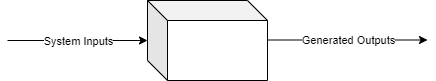
\includegraphics[scale=0.65]{images/functional_inputs_outputs.png}
    \caption{Blackbox testing}
    \label{fig:ast_class_diagram}
\end{figure}

The Cause-Effect Graph (CEG) technique is a black-box method that considers only the desired external behavior of a system. It is also the only black-box test design technique that considers combinations of causes of system behaviors \cite{nursimulu_cause-effect_1995}.

It can be assumed that each requirement in the form of \textit{GIVEN WHEN THEN} dictate a cause effect, as such, a collection of requirements cover a certain area of the software.\\

Robustness testing is the ability of a software to keep an "acceptable" behaviour expressed in terms of \textit{robustness requirements}, in spite of exceptional or unforeseen execution conditions, such as communication failures, degraded modes, etc. \cite{khendek_model-based_2005}. Robustness requirements are within the set of pilot Railway project requirement collection, thus, it can be stated that by testing each requirement causes within the scope of this Railway project, Requirement coverage is achieved.\\

As previously stated, a Requirement \textit{GIVEN} predicate defines the requirement or test pre-conditions, and \textit{WHEN} defines the requirement trigger conditions and implies an internal state change, thus, by invalidating such requirement conditions does not guarantee that the system or software internal state is changed and system behaves otherwise.\\

For a requirement that implies a change of a state, it needs to verify whether different causes or conditions do not conflict with the current state change. An hypothetically example can be observed on the following image (Fig. \ref{fig:door_isolation}).\\

\begin{figure}[H]
    \centering
    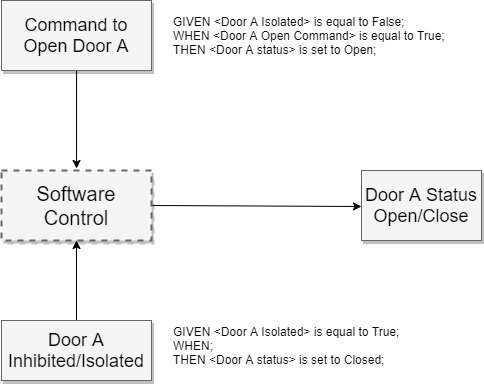
\includegraphics[scale=0.6]{images/isolation_diagram.png}
    \caption{Internal State change - Door Isolation}
    \label{fig:door_isolation}
\end{figure}

In the above example (Fig. \ref{fig:door_isolation}), the Door Isolation requirement when evaluating to true needs to guarantee that the Door close state is assured, however, it cannot be stated otherwise, i.e., that door state would be set to Open when Isolation is not present, as this is given by the Door Open command, this requirement needs to verify that there are no other conditions conflicting or affected the desired results, hence, the verification of the presence of the isolation.

In summary, \textit{Sesnando} generates test cases according to requirement instructions.\\

On an additional note, an internal survey has been revealed that conflicting requirements are very unlikely to happen, however, for cases where it does, those should be found on \textit{upper} vehicle/system level testing.\\

\textcolor{red}{Provision - Se o Sesnando suportar opcionalmente negative tests a partir de AND requirements, ou seja, quando não existem requisitos de robustez, falar disso aqui.}\\


\subsection{Signal Manager Architecture}
%----------------------- Signal manager ----------------------------
\label{subsec:method_signal_manager}

As previously stated, it is intended that Signal Manager could be run as a detached service from the local compiler solution. This would allow that every tester, developer or involved user could contribute to the growth of information in it, such that, every piece of testing information needed would be added only once, thus, the Test Generator accesses this remote repository in order to generate its tests, contributing to efficiently reduce the efforts needed, otherwise, every signal would need to be added as much as every existing localhost solutions.\\
The Signal manager acts as a Web Service and serves the Signal Manager through a REST API. There are several endpoints to consult, edit and create additional signals on the database. The purpose of this API Endpoints is not only to support Test Generator, but also the management of the signal data without the need of accessing the web user interface, e.g, automating the import of huge chunks of signal data. The Signal Manager contains fourteen database tables, next is an excerpt of this database (Fig. \ref{fig:db_signal_manager}) that support the logic described throughout this report.\\

\begin{figure}[H]
    \centering
    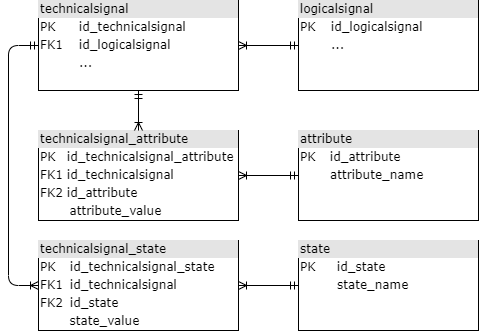
\includegraphics[scale=0.7]{images/signal_manager.png}
    \caption{Signal Manager DB Architecture (Excerpt)}
    \label{fig:db_signal_manager}
\end{figure}

A Logical Signal maps to one or more technical signals and a technical signal supports multiple attributes and states. A train Brake can be used as an example, as a possible attribute would be the location of this Brake within the train (Car=1,2..N) and its Axle (Axle=1..2), given that a train Car might contain two axles and a possible state would be whether this brakes are released or not (state="released", "not released") the latter usually maps to an integer value to represent the state, i.e, 1 or 0. This information is cross-checked on the Test Generator to process the correct technical signals according to the requirement information.


\subsection{Test Designer}
%----------------------- Signal manager ----------------------------
\label{subsec:method_signal_manager}

The main benefits the test designer is the ability of the user to visualise the contents the test specification. By default, the test generator persists the test specification on a CSV file, so, without a Graphical User Interface, the user would have to rely on external tools in order to review it. In other words, the Test Designer loads the CSV contents into a grid-view where several operations might be executed, such as editing and saving this CSV file or generate test scripts.
